% don't remove the folling lines, and edit the defintion of \main if needed
\documentclass[../report.tex]{subfiles}
\providecommand{\main}{..}
\IfEq{\jobname}{\currfilebase}{\AtEndDocument{\biblio}}{}
% until here

\begin{document}

\section{Electroweak symmetry breaking and new resonances}
\label{sec:BSM-EWKNR}

\subsection{Contact interactions}
\label{sec:contactint}

Higher-dimensional operators in an EFT are the most robust and model-independent way of describing BSM virtual effects whenever there is a large separation between the EW and new-physics mass scales. The only drawback of this approach is that, without any theoretical bias on the underlying BSM model, one is confronted with a large number of independent operators, all compatible with SM symmetries. Here, representative sets of operators, which are typically generated in BSM extensions of the EW symmetry breaking (EWSB) sector and which allow for an informative comparison between different collider facilities, are considered.

As a first example, consider the operators ${\cal O}_{2W}$ and ${\cal O}_{2B}$ (defined in ref.~\cite{Giudice:2007fh}), which correspond to the oblique parameters $W$ and $Y$~\cite{Barbieri:2004qk} and describe the leading higher-derivative corrections to the SM gauge boson propagators. Using the equations of motion, these operators lead to charged and neutral current {\it four-fermion contact interactions} of universal type.
The 95\% CL exclusion reach of different colliders on the effective scales of the operators ${\cal O}_{2W}$ and ${\cal O}_{2B}$ is shown in Fig.~\ref{fig:4f}. The precise definition of each collider option is given in ref.\cite{deBlas:2019rxi}. In some cases (ILC, CLIC, FCC) different phases or running modes of the same collider program are shown. All collider sensitivities shown in Fig.~\ref{fig:4f} are derived after combination with the results expected from the HL-LHC, which will precede all future colliders. 
The projected limits come from a variety of di-fermion final states. 
Lepton colliders with suitable luminosity are particularly powerful in testing the neutral-current case thanks to the clean signatures, the small theoretical uncertainties, and the capability to perform detailed differential analyses for a large set of di-fermion final states. The reach of the FCC-ee and CEPC shown in the figure should be considered as slightly underestimated with respect to expectations, due to the absence in the current ESPP inputs of dedicated studies of di-fermion production above the Z pole. Linear colliders can also benefit from different longitudinal polarisations of the two beams.
Hadron colliders have the additional advantage of excellent sensitivity via Drell-Yan (DY) production for both neutral and charged currents, because of the accessible charged initial states (e.g.  $u\bar{d}$). As a matter of fact, the reach of hadron colliders for charged and neutral currents is expected to be about the same. The apparent exception for the HE-LHC collider is simply due to the absence of dedicated charged Drell-Yan studies in the present inputs. As expected for contact interactions, the experimental sensitivity increases significantly with $\sqrt{s}$ in all cases. The results from $ep$ colliders are not shown because they are not competitive: LHeC does not improve the reach of HL-LHC, and FCC-eh does not affect the global fit of FCC-ee/hh.

\begin{figure}[htb]
%\begin{figure}[t]
    \centering
    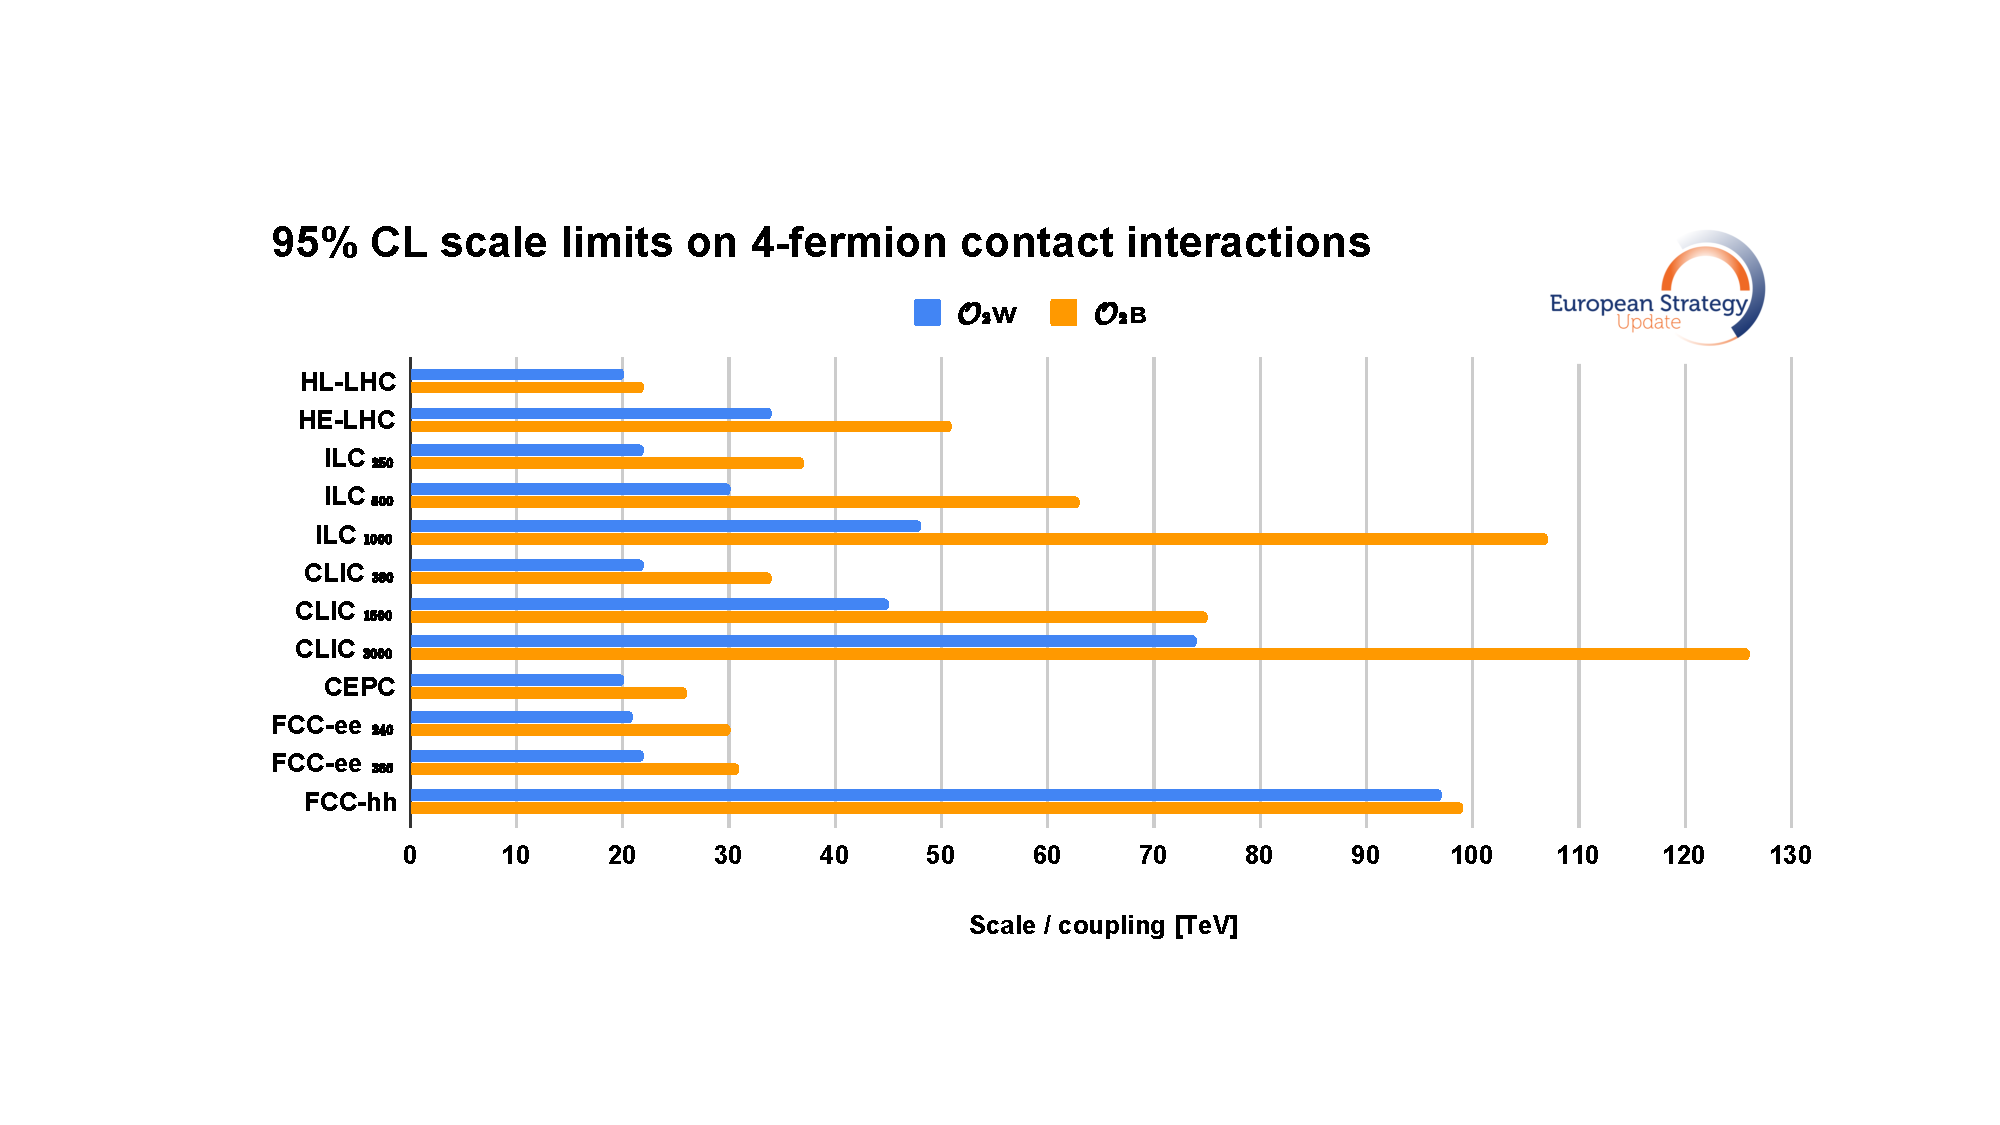
\includegraphics[width=1.0\textwidth]{\main/BSM/EWSB/plots_EWSB/4-fermion-Contact-Interactions.pdf}
    \caption{Exclusion reach of different colliders on four-fermion contact interactions from the operators $\mathcal{O}_{2W}$ and $\mathcal{O}_{2B}$. The blue bars give the reach on the effective scale $\Lambda /(g_2^2 \sqrt{c_{2W}})$ and the orange bars on $\Lambda /(g_1^2 \sqrt{c_{2B}})$, where $c_{2W,2B}$ are the Wilson coefficients of the corresponding operators and the gauge couplings come from the use of the equations of motion.}
    \label{fig:4f}
\end{figure}

As a second example, consider the operators ${\cal O}_{W}$ and ${\cal O}_{B}$ (defined in ref.~\cite{Giudice:2007fh}), which are of special phenomenological relevance for BSM theories of EWSB because they describe new-physics effects in the interaction between the gauge and Higgs sectors. Using the equations of motion, they can be turned into {\it two-fermion/two-boson contact interactions}. The reach on the effective scales of the operators ${\cal O}_{W}$ and ${\cal O}_{B}$ is shown in Fig.~\ref{fig:2f2b}. The projected limits come from new-physics contributions that can interfere with SM di-boson production processes. For CLIC, the leading sensitivity on ${\cal O}_{W}$ comes from a detailed differential analysis of ${e^+e^-}\to {ZH}$~\cite{Beneke:2014sba}, whereas the power of FCC-hh comes through an analysis of the $p_T$ distribution of the $Z$ in ${pp}\to {WZ}$~\cite{Franceschini:2017xkh}. The largest sensitivity of lepton colliders at lower $\sqrt{s}$ and even on the ${\cal O}_{B}$ operator alone at large $\sqrt{s}$ comes from EW precision measurements of the oblique parameter $S$, which constrains directly the combination ${\mathcal{O}}_{W}+{\mathcal{O}}_{B}$~\cite{Giudice:2007fh}. It is also noted that the potential of the ILC$_{1000}$ collider option shown Fig.~\ref{fig:2f2b} should be considered as slightly underestimated, due to the absence of dedicated  differential ${e^+e^-}\to {ZH}$ results in current inputs.


\begin{figure}[htb]
%\begin{figure}[t]
    \centering
          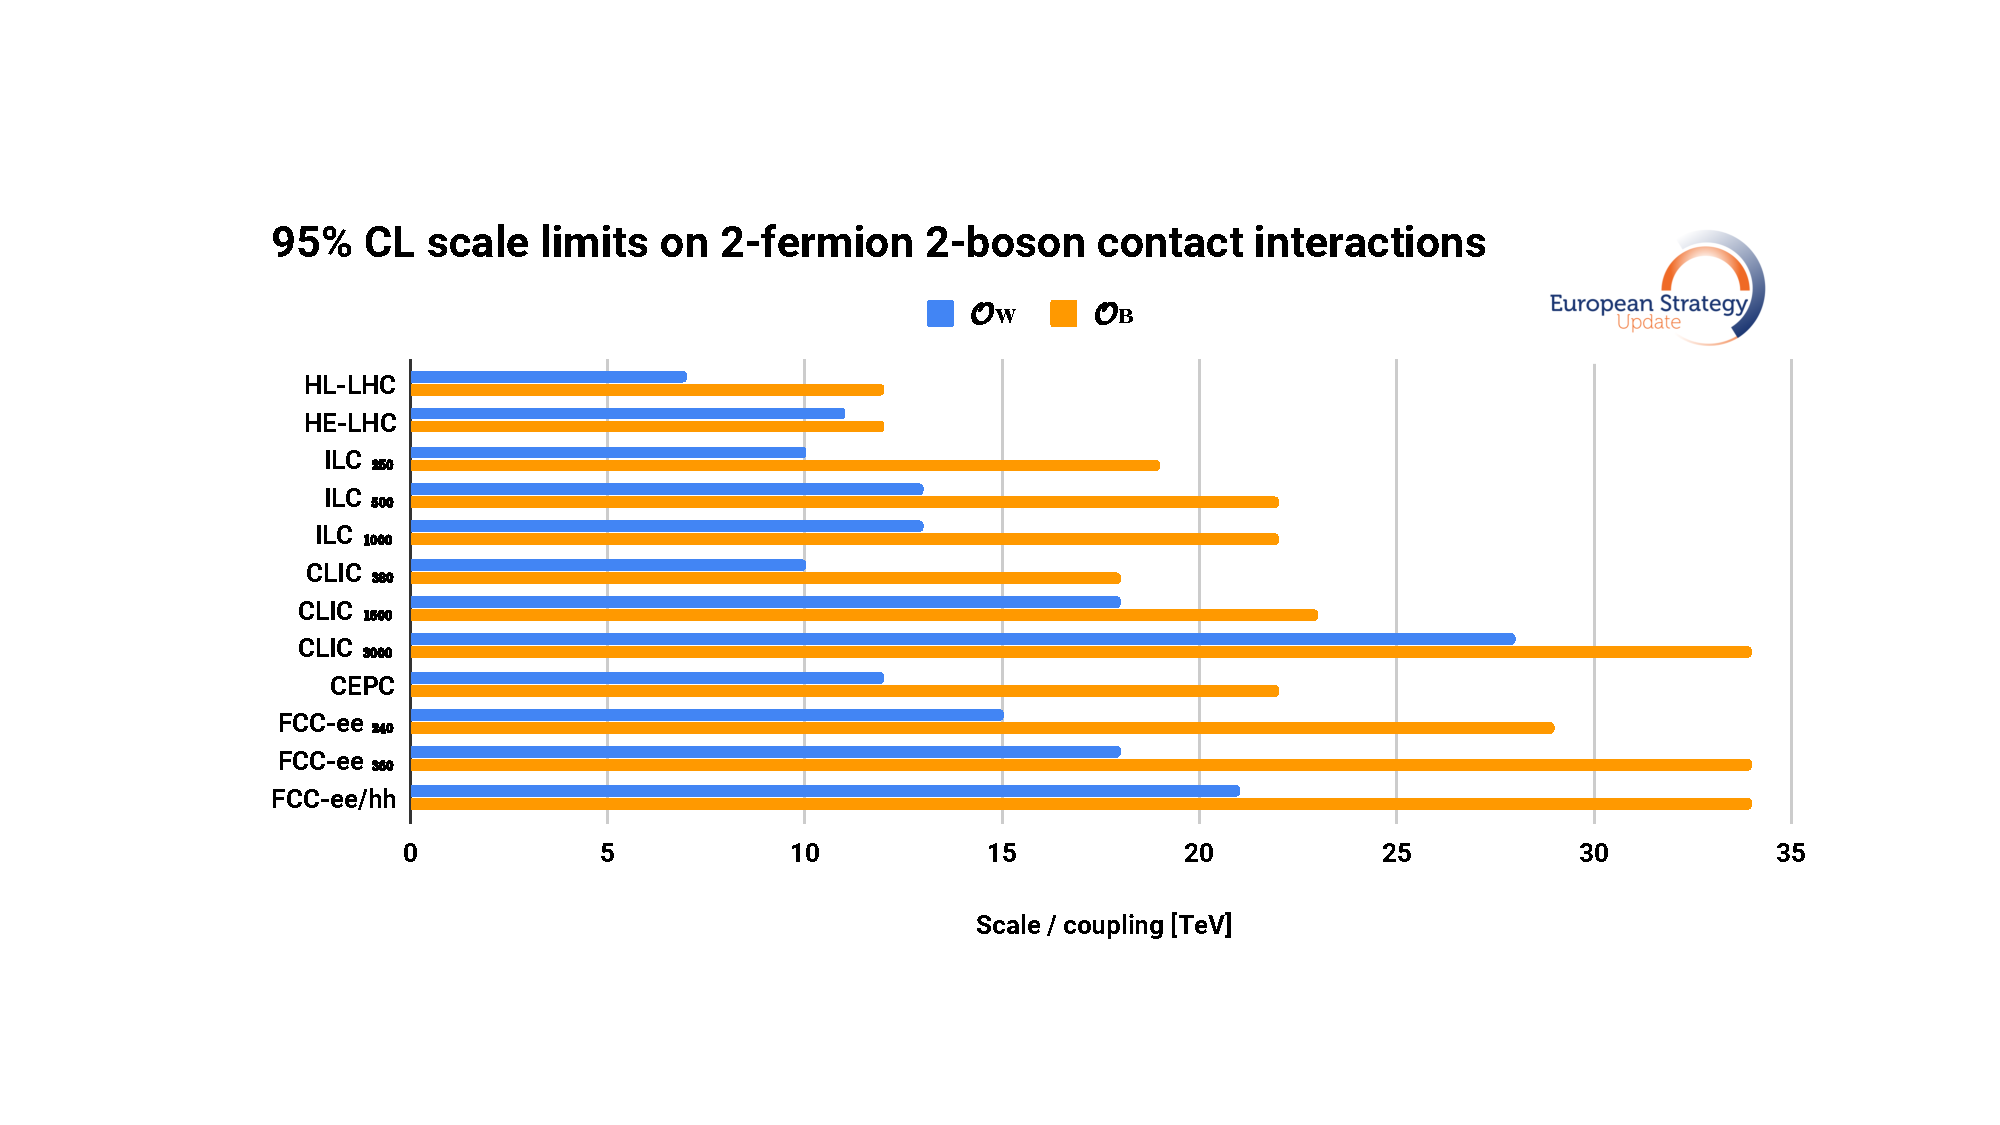
\includegraphics[width=1.0\textwidth]{\main/BSM/EWSB/plots_EWSB/2-fermion-2-boson-Contact-Interactions.pdf}
    \caption{Exclusion reach of different colliders on the two-fermion/two-boson contact interactions from the operator $\mathcal{O}_{W}$ and $\mathcal{O}_{B}$. The blue bars give the reach on the effective scale $\Lambda /(g_2^2 \sqrt{c_{W}})$ and the orange bars on $\Lambda /(g_1^2 \sqrt{c_{B}})$, where $c_{W,B}$ are the Wilson coefficients of the corresponding operators and the gauge couplings come from the use of the equations of motion.}
    \label{fig:2f2b}
\end{figure}

\subsection{New vector bosons: the $Y$-Universal $Z^\prime$}

New vector bosons are common in many BSM theories, ranging from new models of EWSB to extensions of the SM gauge group. As a representative example of these classes of theories, the ``$Y$-Universal $Z^\prime$'' (see e.g. \cite{Appelquist:2002mw}) is considered. The model consists of a new neutral gauge boson $Z^\prime$ with mass $M$ and charges to SM particles equal to hypercharge, although the coupling constant $g_{Z^\prime}$ is taken to be a free parameter, in general different from the one of the SM \mbox{U$(1)_Y$}. The perturbative limit is taken to correspond to $g_{Z^\prime}<1.5$ since for larger values the width of the $Z^\prime$ exceeds $0.3\, M$.

The $Y$-Universal $Z^\prime$ is selected instead of one of the standard benchmarks (such as the Sequential or $B-L$ models) for several reasons. It has comparable couplings to quarks and leptons, allowing for a fair comparison between hadron and lepton colliders. Its couplings are flavour-diagonal, making the model safely compatible with flavour constraints. When integrated out at tree-level, it generates only the universal operator ${\mathcal{O}}_{2B}$ in the SM EFT, with coefficient ${c_{2B}}/{\Lambda^2}={g_{Z^\prime}^2}/{(g_1^4 M^2)}$.  Since the sensitivity to ${\mathcal{O}}_{2B}$ is available for all colliders~\cite{deBlas:2019rxi}, a straightforward and rigorous assessment of the indirect reach is possible for the $Y$-Universal $Z^\prime$ model, while additional input would be needed for the standard benchmarks.

Figure~\ref{fig:Universal_Zp} displays the $95\%$~CL exclusion reach on $g_{Z^\prime}$ and $M$, at various colliders. For hadron machines, the reach of direct searches (round curves at small $g_{Z^\prime}$) is obtained from recasting the results in Refs.~\cite{CidVidal:2018eel,Jamin:2019mqx}, overlaid with the indirect sensitivity (diagonal straight lines at large $g_{Z^\prime}$) discussed previously. It is seen that the direct mass reach is inferior to the indirect one for high $g_{Z^\prime}$, in agreement with the generic expectation that strongly-coupled new physics is better probed indirectly. Moreover, the indirect reach  benefits greatly from higher collider energies. These two observations explain both the competitiveness of lepton colliders in indirect searchesand  the good indirect performances of the FCC-hh and HE-LHC colliders.

\begin{figure}[t]
    \centering
    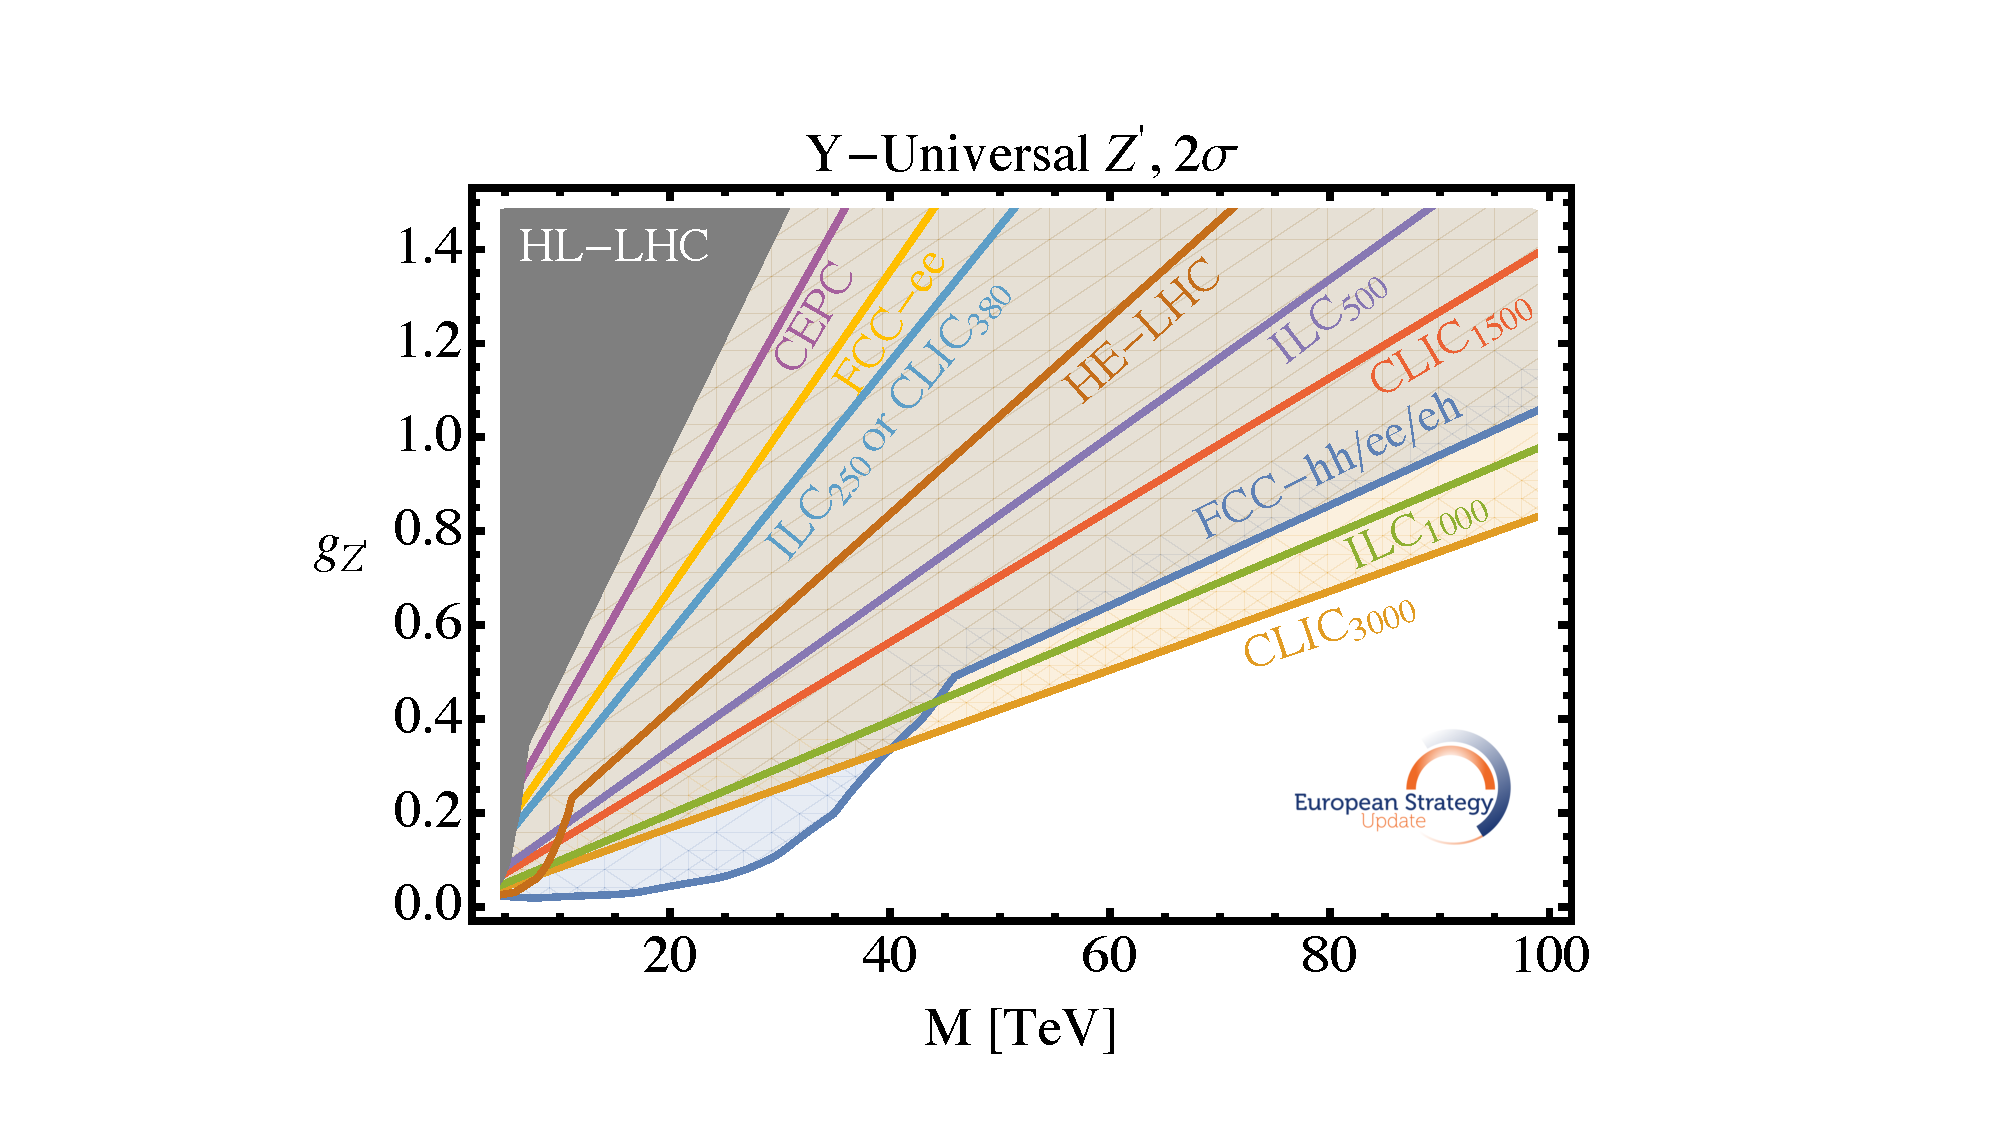
\includegraphics[width=0.6\textwidth]{\main/BSM/EWSB/plots_EWSB/Y-Universal.pdf}
    \caption{Exclusion reach of different colliders on the $Y$-Universal $Z^\prime$ model parameters. The gap in performances between CEPC or FCC-ee with respect to ILC$_{250}$ or CLIC$_{380}$ is most likely due to the lack of dedicated di-fermion production studies as discussed in Sect.~\ref{sec:contactint}.}
    \label{fig:Universal_Zp}
\end{figure}

\subsection{The Composite Higgs scenario}

Decades of theoretical investigation (for a review, see \cite{Panico:2015jxa}) provided us with a rather clear picture of how a viable Composite Higgs model should look like, and with effective parametrisations of the relevant phenomenology that can be employed in the present context. The central idea is that the Higgs emerges as a bound state of a new strongly-interacting confining Composite Sector, analogue to QCD but with a much higher confinement scale. The Higgs, similarly to the pions in QCD, emerges as a Goldstone boson associated with a spontaneously-broken global symmetry of the Composite Sector. This explains why it is lighter than other bound states (collectively called `resonances') that will unavoidably emerge from the Composite Sector dynamics. In analogy with the pion in QCD, the spin-one resonances will be called $\rho$.

The phenomenology is mainly controlled by two parameters: the mass scale $m_*$ and the coupling $g_*$. The mass $m_*$ is the Composite Sector confinement scale, analogue to $\Lambda_{\rm{QCD}}$. It controls the mass of the resonances and sets the scale of the EFT operators that describe at low energy the indirect effects of Higgs compositeness. Its inverse can be interpreted as the \emph{geometric size} of the Higgs, $\ell_H=1/m_*$. The sensitivity of future colliders to $\ell_H$ is the most important parameter to answer the question whether the Higgs is elementary ($\ell_H=0$) or composite ($\ell_H\neq0$). The coupling parameter $g_*$ represents the interaction strength among particles originating from the Composite Sector. It controls the strength of the Higgs couplings to the $\rho$ resonance and it sets the scale of couplings that appear in the EFT Lagrangian. The internal coherence of the construction requires $g_*$ to be larger than the EW coupling ($g_*\gtrsim 1$) but smaller than the perturbative unitarity limit ($g_*\lesssim 4\pi$). 

Among the operators in the Composite Higgs EFT,  $\mathcal{O}_{\phi}$ (defined as in \cite{deBlas:2019rxi}), $\mathcal{O}_{W}$ and $\mathcal{O}_{2W}$ are the most representative and offer the best sensitivity at all colliders. Parametrically, their Wilson coefficients are
\begin{equation}\label{eq:CHOp}
\frac{c_{\phi}}{\Lambda^2}\sim \frac{g_*^2}{m_*^2}\,,\;\;\;\;\;
\frac{c_{W}}{\Lambda^2}\sim \frac{1}{m_*^2}\,,\;\;\;\;\;
\frac{c_{2W}}{\Lambda^2}\sim \frac{1}{g_*^2m_*^2}\,.
\nonumber
\end{equation}
These relations are merely \emph{estimates} of the expected magnitude of the Wilson coefficients, which hold up to model-dependent order-one factors. In the current analysis, these relations are taken as exact equalities, so the results should not be interpreted as strictly quantitative, but only as a fair assessment of the sensitivity. 

\begin{figure}[t]
    \centering
    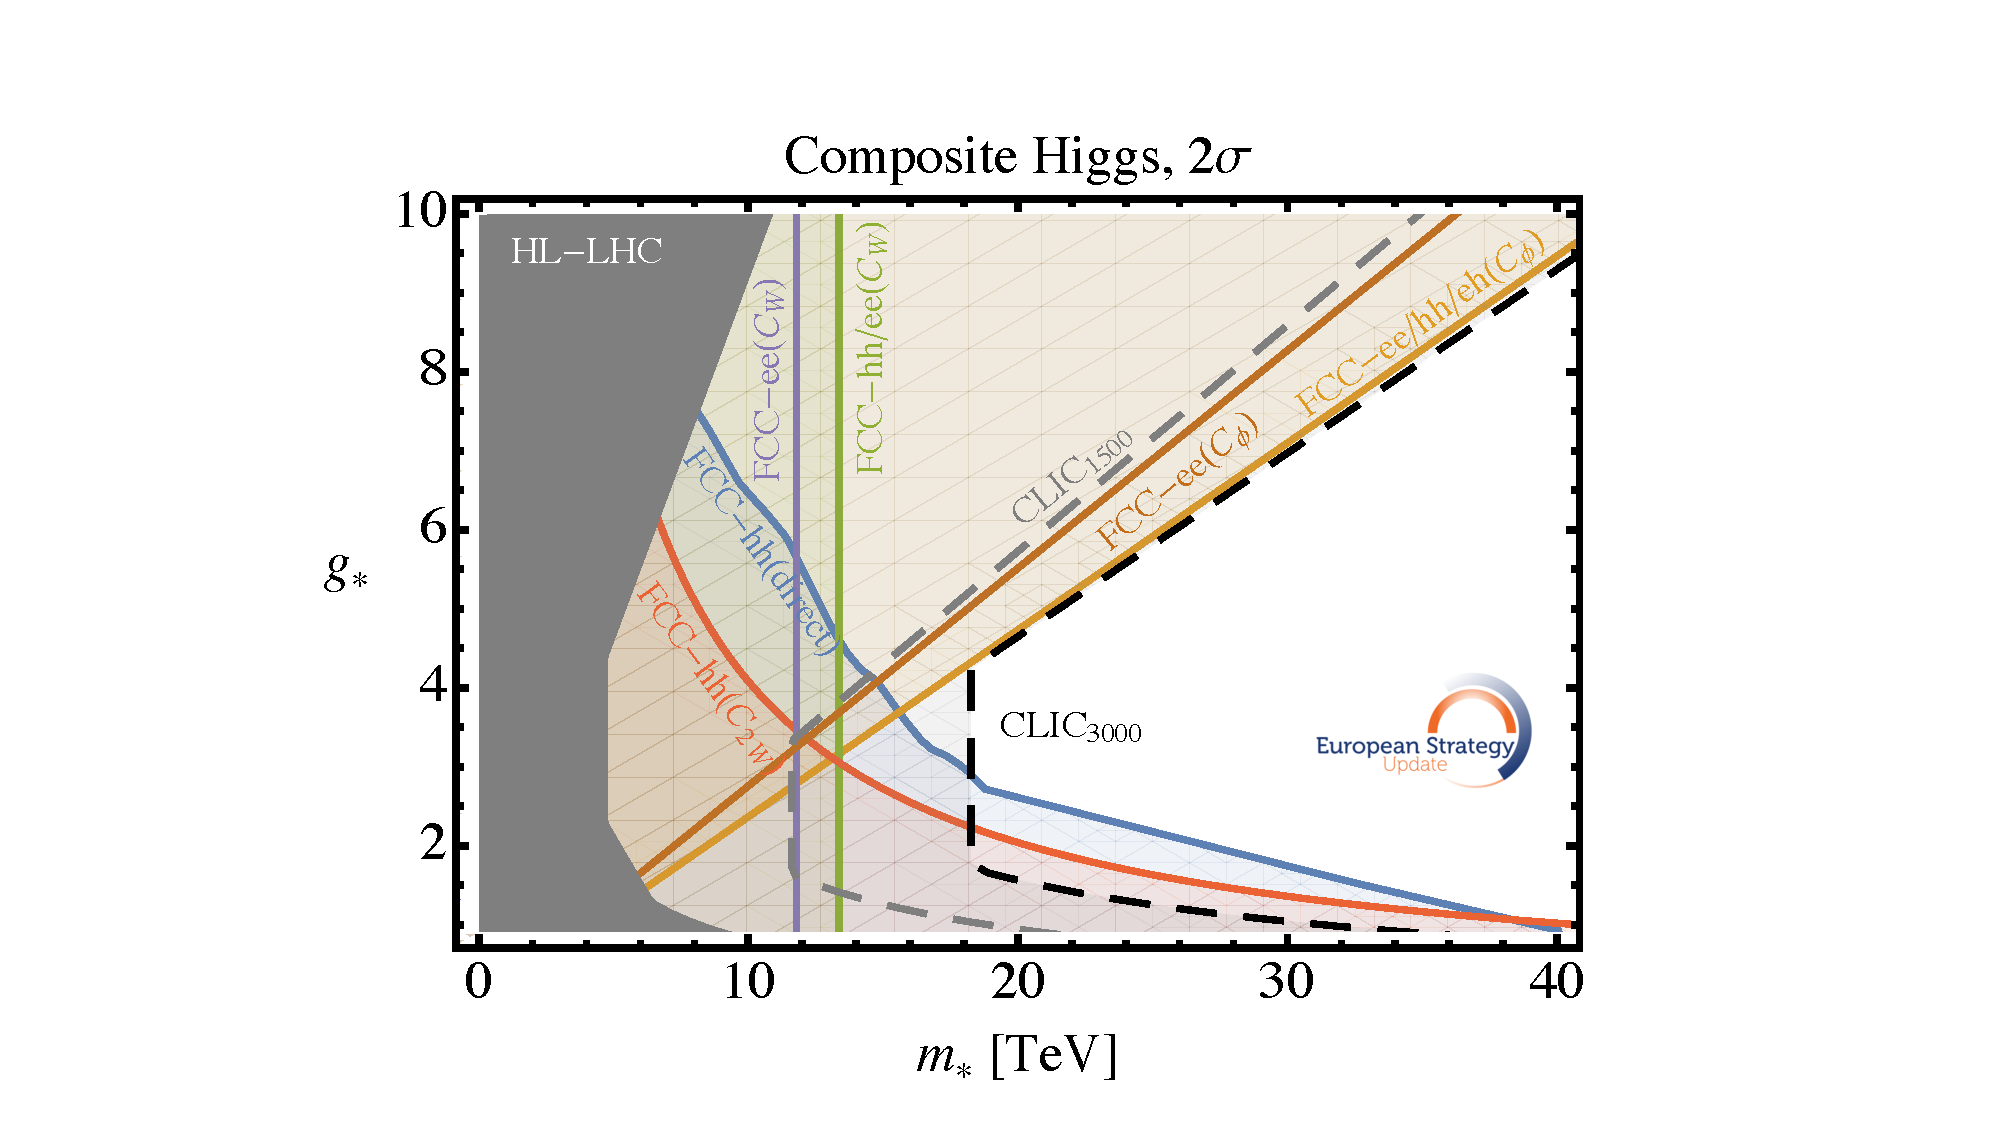
\includegraphics[width=0.48\textwidth]{\main/BSM/EWSB/plots_EWSB/FCCvsCLIC_CH} ~
        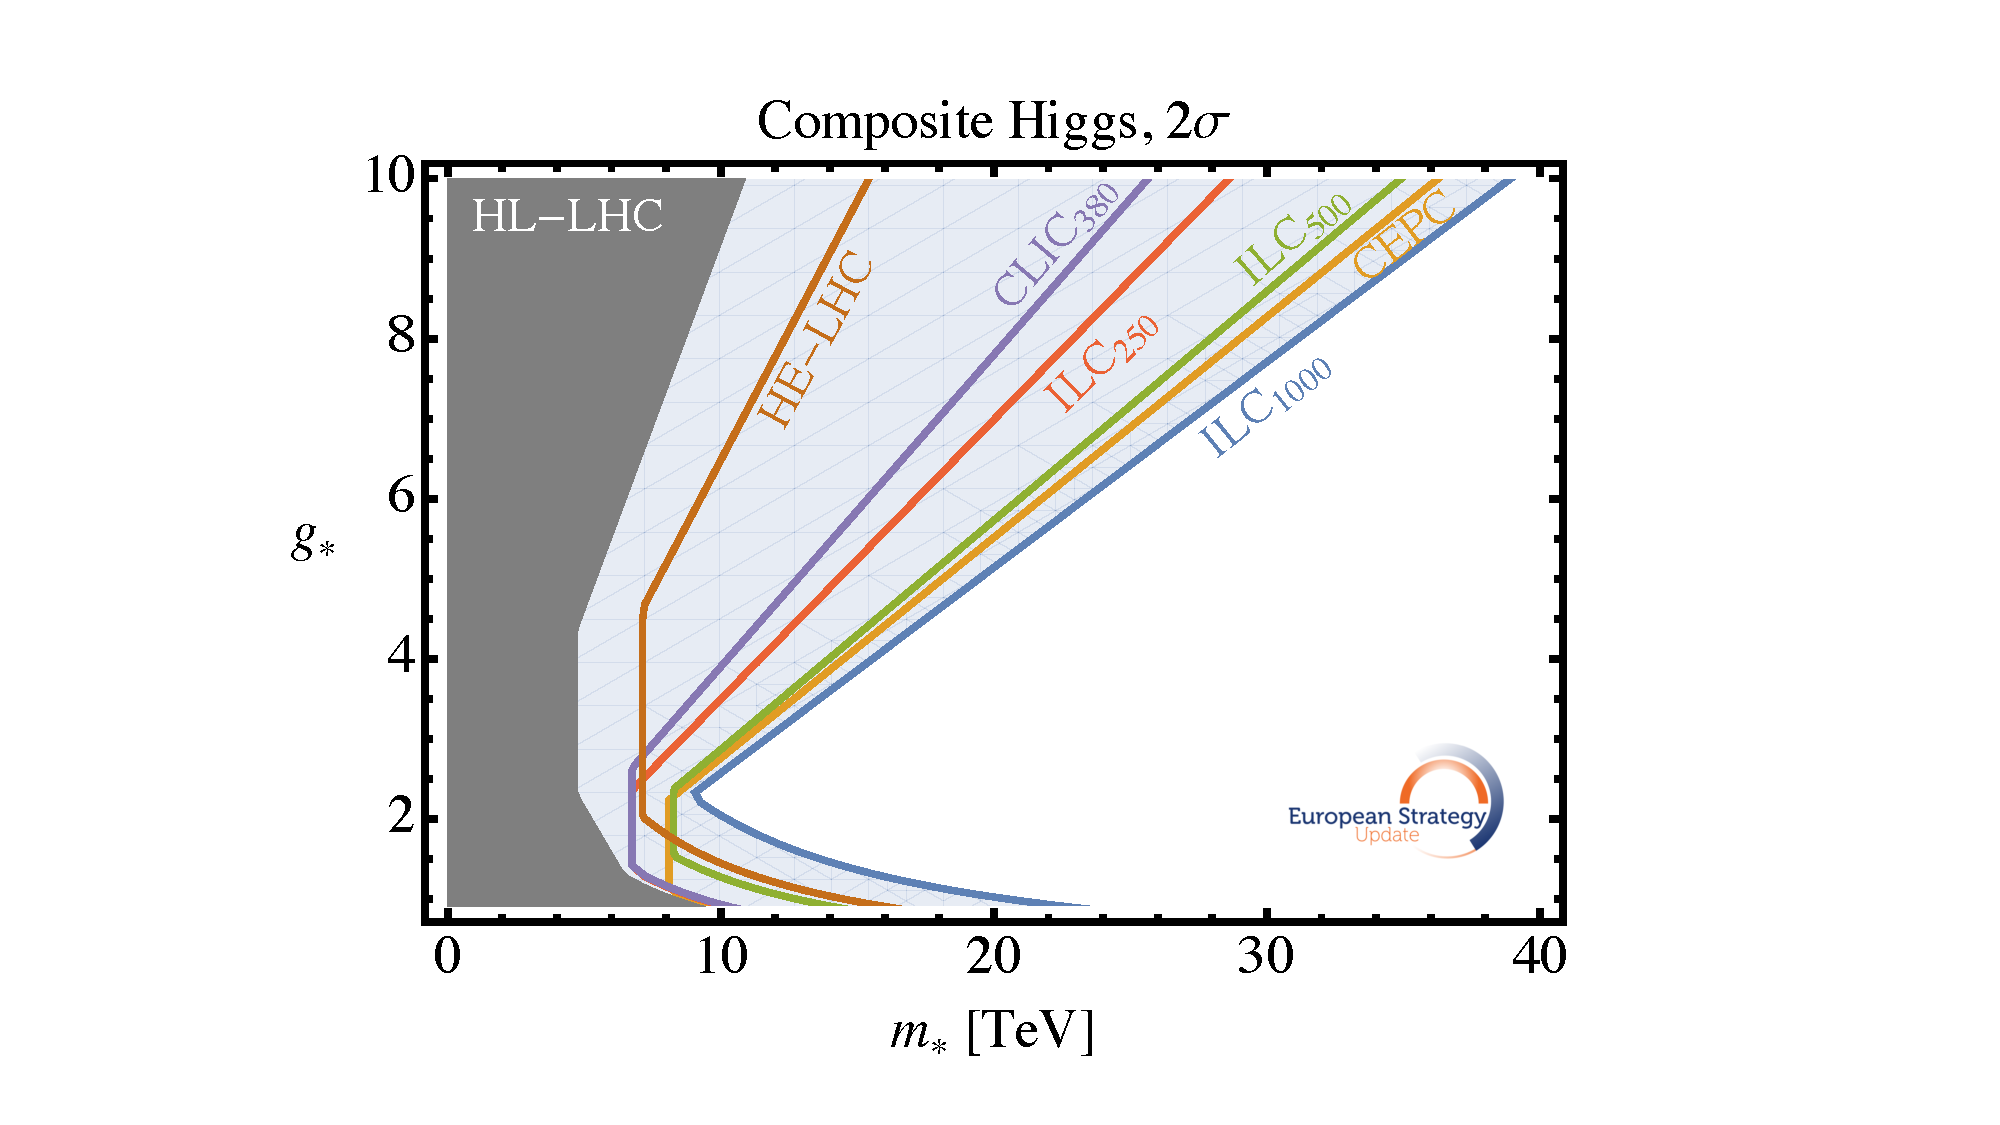
\includegraphics[width=0.48\textwidth]{\main/BSM/EWSB/plots_EWSB/ILCvsCEPC_CH}
    \caption{Left panel: exclusion reach on the Composite Higgs model parameters of FCC-hh, FCC-ee, and of the high-energy stages of CLIC. Right panel: the reach of HE-LHC, ILC, CEPC and CLIC$_{380}$. The reach of HL-LHC is the grey shaded region.}
    \label{fig:Composite_Higgs}
\end{figure}

Figure~\ref{fig:Composite_Higgs} shows the exclusion reach on $m_*$ and $g_*$ from the highly complementary probes on the operators $\mathcal{O}_{\phi}$, $\mathcal{O}_{W}$ and $\mathcal{O}_{2W}$ with different experimental strategies in different colliders. For the FCC project, $\mathcal{O}_{\phi}$ is most effective at large $g_*$, and it is well probed by Higgs couplings measurements at FCC-ee. However FCC-hh and FCC-eh further improve the reach on $c_\phi$ as shown in the figure. The reach on $c_\phi$ for all collider options is extracted from the summary Table~8 of Ref.~\cite{deBlas:2019rxi}, with the exception of HL-LHC for which a more conservative value of $c_\phi|_{1\sigma}=0.42/{\rm{TeV}}^2$ (also reported in Ref.~\cite{deBlas:2019rxi}) is employed. The operator $\mathcal{O}_{2W}$ is instead effective at low $g_*$, and it is probed by high-energy charged DY measurements at FCC-hh~\cite{Farina:2016rws}. The mass-reach from $\mathcal{O}_{W}$ is instead independent of $g_*$.  The reach of direct resonance searches is also shown in Fig.~\ref{fig:Composite_Higgs}, for the \FCChh and the \HLLHC. It represents the sensitivity to an EW triplet $\rho$ vector resonance, generically present in Composite Higgs models. The reach is extracted from ref.~\cite{Thamm:2015zwa,Golling:2016gvc,Mangano:2651294}, and it emerges from a combination of dilepton and diboson final state studies. Direct searches are more effective at \emph{low} $g_*$, which may seem surprising. The reason is that $g_*$ is the $\rho$ coupling to the Higgs boson, while the coupling of the $\rho$ to quarks, which drives the production, scales like $g_2^2/g_*$ and therefore increases for small $g_*$. Unfortunately, no direct reach projection is currently available for the \HELHC.

The information in Fig.~\ref{fig:Composite_Higgs} can be projected into a single number, as displayed in Fig.~\ref{fig:Composite_Higgs_Summary}. The orange bars show the maximum $m_*$ (or, equivalently, the minimum Higgs size $\ell_H$) a given collider is sensitive to, independently of the value of $g_*$. The purple bars show the tuning parameter $1/\epsilon$ (which is equal to the conventional tuning parameter $\Delta$), obtained as follows. Higgs compositeness can address the naturalness problem, provided it emerges at a relatively low scale, but the parameter $m_*$ is not the most appropriate measure of the degree of fine-tuning required to engineer the correct Higgs mass and EWSB scale. A better measure is (see e.g., \cite{Matsedonskyi:2015dns}) $1/\epsilon>(m_T/500\,{\rm{GeV}})^2>m_*^2/g_*^2v^2$,
where $v=246$~GeV and $m_T$ is the top-partner mass. The second inequality provides the estimate of the reach on $\epsilon$ reported in Fig.~\ref{fig:Composite_Higgs_Summary}. The equation also displays the impact of fermionic top-partner searches on $\epsilon$. The discovery reach of these particles at HL-LHC, HE-LHC and FCC-hh are of $1.5$, $2$ and $4.7$~TeV, respectively. These correspond to a reach on $1/\epsilon$ of $10$, $16$ and $88$.

\begin{figure}[t]
    \centering
    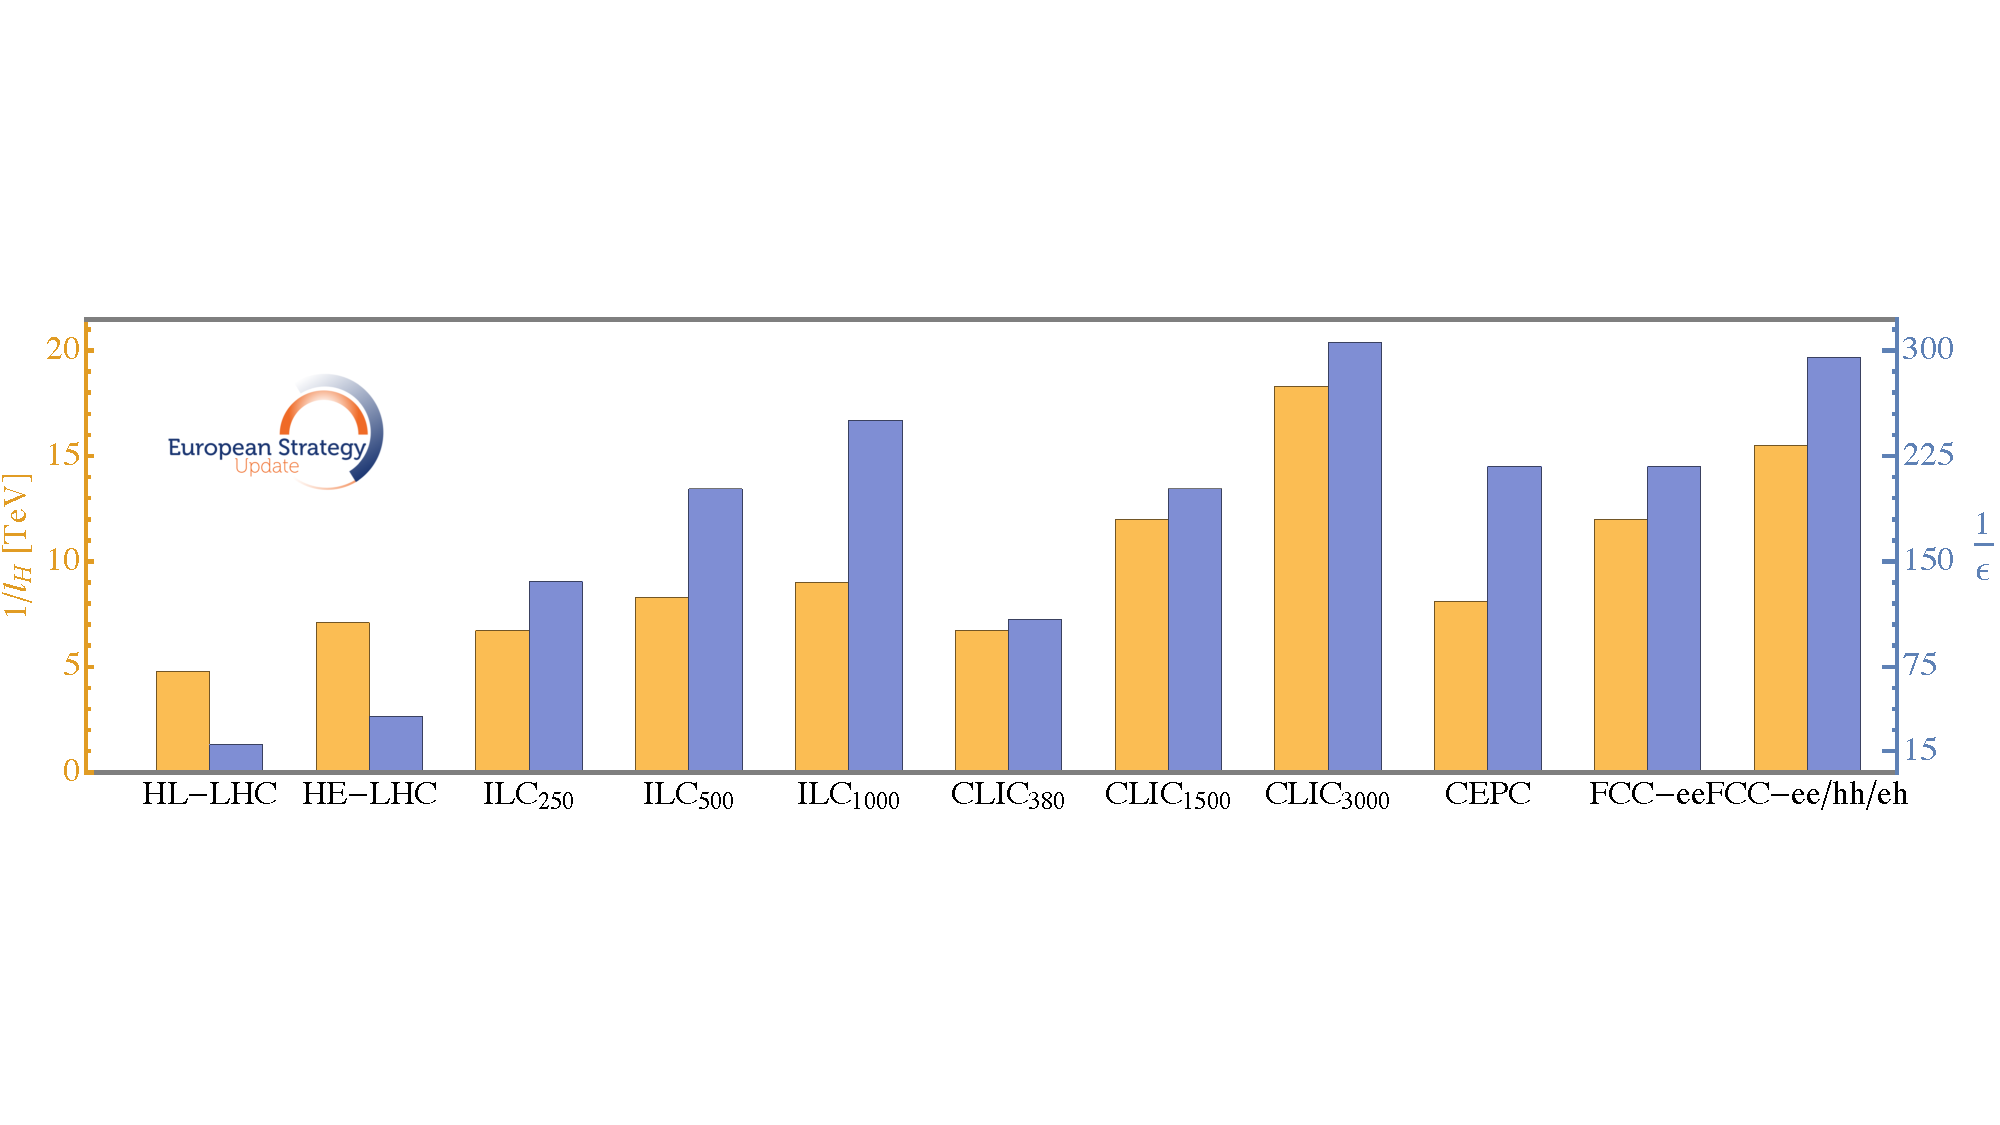
\includegraphics[width=1.0\textwidth]{\main/BSM/EWSB/plots_EWSB/Length_and_Tuning}
    \caption{Exclusion reach of different colliders on the inverse Higgs length $1/\ell_H =m_*$ (orange bars, left axis) and the tuning parameter $1/\epsilon$ (blue bars, right axis), obtained by choosing the weakest bound valid for any value of the coupling constant $g_*$. The $m_*$ reach of the ILC is underestimated because of the lack of a dedicated $\mathcal{O}_{W}$ analysis in the $ZH$ final state as explained in Sect.~\ref{sec:contactint}.}
    \label{fig:Composite_Higgs_Summary}
\end{figure}

\end{document}


